\documentclass{VUMIFPSkursinis}
\usepackage{algorithmicx}
\usepackage{algorithm}
\usepackage{algpseudocode}
\usepackage{amsfonts}
\usepackage{amsmath}
\usepackage{bm}
\usepackage[margin=50pt]{caption}
\usepackage{color}
\usepackage{float}
\usepackage{graphicx}
\usepackage{listings}
\usepackage{subfig}
\usepackage{wrapfig}
\usepackage{fontspec}
\usepackage{todonotes}
\usepackage{pdfpages}
%\newcommand{\TD}[1]{\todo[inline, color=red!40]{#1}}

% Titulinio aprašas
\university{Vilniaus universitetas}
\faculty{Matematikos ir informatikos fakultetas}
\department{Programų sistemų bakalauro studijų programa}
\papertype{Kursinis darbas}
\title{Raft Algoritmo Ra Praplėtimų Tyrimas}
\titleineng{Investigation of Raft Algorithm Ra Extensions}
\status{3 kurso 1 grupės studentas}
\author{Edvardas Dlugauskas}
% \secondauthor{Vardonis Pavardonis}   % Pridėti antrą autorių
\supervisor{dr. Karolis Petrauskas}
\date{Vilnius – \the\year}

% Nustatymai
\setmainfont
[Path = ./palem/,
 Extension = .ttf,
 UprightFont = *-nm,
 BoldFont = *-bd,
 ItalicFont = *-it,
 BoldItalicFont = *-bi]
{Palem}
\bibliography{bibliografija}

\begin{document}
\maketitle
% \listoftodos
\tableofcontents

\sectionnonum{Įvadas}

Mūsų amžiuje, esminėms visuomenės sistemoms persikeliant į virtualią erdvę, informacinių sistemų stabilumas tampa vis svarbesnis. IT sistemos turi atlaikyti aparatinės įrangos gedimus, nes vieno bito apvertimas sistemos kūrėjams gali kainuoti labai daug. Neseniai atliktas tyrimas parodė, kad apie 8\% visų serverių gali tikėtis per metus patirti bent vieną sutrikimą~\cite{characterizing_cloud_hardware_rel}.

Paskirstytos sistemos yra patraukli alternatyva lygiagrečioms sistemoms, leidžianti efektyviai panaudoti šiuolaikiškus IT resursus ir užtikrinti sistemos gyvybingumą ir korektiškumą~\cite{steen_distributed_2017, ongaro_consensus}. Viena iš esminių paskirstytų sistemų problemų yra konsensuso pasiekimas. Paskirstytos sistemos veikimo metu gali būti situacijų, kai kelių mazgų būsenos yra skirtingos. Pavyzdžiui, kai vienas iš mazgų trumpam laikui tampa neprieinamas ir negali atnaujinti savo būsenos, o vėliau vėl tampa prieinamas. Mazgų būsenos gali išsiskirti, ir iš skirtingų mazgų klientui gali būti grąžinami skirtingi rezultatai. Tai pažeistų sistemos vientisumą. Todėl būtina sinchronizuoti būsenas tarp mazgų ir tuo pačiu metu leisti sistemai veikti toliau jei pakankamai maža dalis mazgų neveikia ar yra nepasiekiama. Tam reikia išspręsti konsensuso problemą -- kaip mazgai gali pasiekti susitarimą dėl jų bendros būsenos, net kai dalis mazgų gali būti nepasiekiama ar jos duomenys pasenę?

Formaliai, paskirstyta sistema yra skaičiavimų elementų (toliau - mazgų) rinkinys, kuris yra naudojamas kaip vientisa sistema~\cite{steen_distributed_2017}. Paskirstytose sistemose konsensuso algoritmai yra reikalingi būsenų sinchronizavimui tarp sistemos mazgų. Konsensuso algoritmas turi užtikrinti, kad sistema būtų prieinama vieno ar daugiau mazgų gedimo ar neprieinamumo atvejais~\cite{ongaro_consensus}. 

Šiame darbe išnagrinėti Raft konsensuso algoritmo praplėtimai naudojami Ra bibliotekoje. Raft yra konsensuso algoritmas sukurtas palengvinti konsensuso algoritmų įgyvendinimo naštą sistemų architektams ir leisti lengvai praplėsti ir pritaikyti Raft algoritmą specifinėms reikmėms~\cite{ongaro_consensus}. 

Šio darbo tikslas yra patikrinti, ar Raft algoritmas, praplėstas Ra naudojamais mazgų neveikimo aptikimo praplėtimais, vis dar atitinka Raft algoritmo savybes ir užtikrina efektyvų mazgų neveikimo aptikimą~\cite{ongaro_consensus, rabbitmqra}.

Šio darbo uždaviniai yra:
\begin{itemize}
    \item Išnagrinėti Raft algoritmą ir biblioteką Ra.
    \item Pateikti esamos literatūros apie Raft algoritmą ir Ra įgyvendinimo apžvalgą.
    \item Išanalizuoti Ra padarytus praplėtimus ir jų įtaką Raft algoritmui.
    \item Pateikti formalią specifikaciją Ra mazgų neveikimo aptikimui.
\end{itemize}

Šiame darbe parodyta, kad Raft algoritmo bibliotekoje Ra naudojami gimtieji Erlang mazgų neveikimo aptikimo metodai atitinka Raft algoritmo aprašytus širdies plakimo (angl. \textit{heartbeat}) procedūras. Ra suvaldo atvejus, kai mazgas netikėtai nustoja veikti (angl. \textit{crash}), o jei mazgas yra nepasiekiamas ar lėtas, negyvybingumo aptikimo algoritmas atitinka Raft aprašytus scenarijus.

Šis darbas yra paskirstytas į dvi dalis. Pirmoje dalyje yra apžvelgiamas Raft algoritmas ir detaliau išnagrinėjami kelių jo dalių, susijusių su mazgų neveikimo aptikimu, veikimo principai. Antroje dalyje yra aprašomos Raft algoritmo bibliotekoje Ra naudojamos kalbos Erlang ypatybės ir išnagrinėjami Ra padaryti praplėtimai, yra detaliau išnagrinėjami Ra naudojami mazgų neveikimo aptikimo metodai ir jie yra palyginami su Raft pasiūlytu sprendimu.

\section{Raft algoritmo apžvalga}

Raft yra algoritmas, naudojamas konsensusui pasiekti paskirstytoje sistemoje. Bazinio Raft algoritmo  korektiškumas yra įrodytas formalios TLA$^+$ specifikacijos pagalba~\cite{ongaro_consensus} ir naudojimu industrijoje -- Raft naudojamas etcd\footnote{https://etcd.io/}, Consul\footnote{https://www.consul.io/docs/internals/consensus.html} ir CockroachDB\footnote{https://www.cockroachlabs.com/docs/stable/architecture/replication-layer.html} projektuose. 

Raft buvo sukurtas kaip lengviau suprantama alternatyva tuo metu labiausiai paplitusiam Paxos\footnote{http://lamport.azurewebsites.net/pubs/paxos-simple.pdf} konsensuso algoritmui~\cite{ongaro_consensus, diego_designing_2016}. Raft autoriai, atlikus vartotojų tyrimą, parodė, kad Raft algoritmas yra lengviau suprantamas negu Paxos, iš ko seka mažesni įgyvendinimo kaštai, mažesnis galimų klaidų skaičius ir paprastesnis bazinio algoritmo praplėtimas~\cite{ongaro_consensus}. Raft leidžia užtikrinti sistemos gyvybingumą ir saugumą kol veikia daugiau negu pusė paskirstytos sistemos mazgų. 

Raft algoritmo kontekste sistema laikoma būsenų mašina, kuri priima iš klientų užklausas su komandų įrašais. Kiekvienas įrašas yra norimos sistemai įvykdyti komandos aprašymas. Įvykdant komandą, sistema pakeičia savo vidinę būseną ir grąžina klientui rezultatą -- savo atnaujintą būseną ar jos dalį. Atitinkamai, paskirstyta sistema susideda iš mazgų, kurie irgi yra būsenų mašinos, turinčios savo įrašų žurnalus ir vidines būsenas. Toks paskirstytos sistemos išdėstymas leidžia pasiekti aukštą gedimų toleravimo ir greičio lygį~\cite{ongaro_consensus, steen_distributed_2017}.

Raft algoritmas remiasi lyderio išrinkimu -- vienas iš mazgų tampa lyderiu, ir yra laikoma, kad lyderio žurnalas yra tiesos šaltinis. Visos klientų užklausos yra siunčiamos lyderiui, kuris persiunčia įrašus kitiems mazgams (sekėjams). Kai dauguma mazgų turi informaciją apie naują įrašą, mazgai užfiksuoja įrašą savo žurnale ir įvykdo įraše nurodytą komandą. Jei nustoja veikti sekėjas, sistema tęsia darbą, kol yra veikiančių mazgų dauguma. Nustojus veikti lyderiui, nesulaukę lyderio gyvumo patvirtinimo, kiekvienas mazgas po atsitiktinio dydžio laiko, pasirinkto iš nustatyto intervalo,  pradeda rinkimus. Rinkimai prasideda kai vienas iš mazgų padidina savo termino (kadencijos) reikšmę ir išsiunčia kitiems mazgams prašymo balsuoti užklausas. Išsirinkus naują lyderį sistemą gali tęsti darbą~\cite{ongaro_consensus}. 

Sistemos mazgai turi laikiną atmintį, kurioje saugo dažnai naudojamą informaciją, ir ilgalaikę atmintį. Ilgalaikė atmintis turi informacijos apie sistemos konfigūraciją, kuri yra reikalinga korektiškam Raft algoritmo veikimui -- mazgai išsaugo savo dabartinį terminą ir už ką jame balsavo. Taip pat ilgalaikėje atmintyje saugomi užfiksuoti įrašai~\cite{ongaro_consensus}.

Raft specifikacija garantuoja kad Raft algoritmas tenkina sekančias savybes~\cite{ongaro_consensus}: 

\begin{enumerate}
\item Lyderio išrinkimas: duotam lyderio terminui galiausiai bus išrinktas ne daugiau kaip vienas lyderis.
\item Lyderio žurnalo uždarumas modifikacijoms: lyderis niekada nekeičia ir netrina įrašų savo žurnale, jis gali tik pridėti naujų įrašų.
\item Žurnalų įrašų atitikimas: jeigu dviejų mazgų žurnalai turi įrašą su tuo pačiu indeksu ir terminu, tai tie įrašai yra lygūs ir visi abiejų žurnalų įrašai iki to indekso yra lygūs.
\item Lyderio žurnalo pilnumas: jeigu žurnalo įrašas buvo užfiksuotas, tai visų sekančių terminų lyderiai turės tą užfiksuotą įrašą savo žurnale.
\item Sistemos kaip būsenos mašinos saugumas: jei mazgas įvykdė žurnalo įrašą, joks kitas mazgas niekada neįvykdys kitokio įrašo su tuo pačiu indeksu.
\end{enumerate}

Toliau detaliau apžvelgiame kaip Raft užtikrina, kad galiausiai būtų išrinktas mazgų lyderis, kaip lyderis perduoda įrašus kitiems mazgams, ir kaip Raft elgiasi nutikus mazgų tinklo trūkiams.

\subsection{Raft lyderio išrinkimas}

Pagal Raft, mazgas--lyderis periodiškai siunčia savo sekėjams tuščias įrašo pridėjimo užklausas (\texttt{AppendEntries}), taip užtikrinant savo ,,širdies plakimą'' (angl. \textit{heartbeat})~\cite{ongaro_consensus}. Jeigu sekėjas kažkurį laiką negauna užklausų iš lyderio, sekėjas pradeda naujus rinkimus ir pasisiūlo kaip kandidatas į naują lyderį. Nuosekliai auganti reikšmė, nurodanti dabartinio lyderio kadencijos numerį, vadinamą \textit{terminu} (angl. \emph{term}), o laikas, po kurio sekėjas pradės naujo termino rinkimus vadinamas \textit{rinkimų laiku} (angl. \textit{election timeout}). Rinkimų laikas yra atsitiktinė reikšmė iš pasirinkto laiko intervalo, kas padeda greičiau išrinkti naują lyderį kai yra daugiau negu vienas kandidatas~\cite{ongaro_consensus}.

Rinkimų pradžioje, sekėjas tampa kandidatu, balsuoja šiame rinkimų termine už save, ir išsiunčia visiems kitiems mazgams prašymo balsuoti užklausas (\texttt{RequestVote}). Mazgas per rinkimų terminą gali balsuoti tik už vieną mazgą. Mazgai balsuoja už pirmą mazgą, kuris šiame termine atsiuntė prašymą balsuoti, arba už save, jei jie ką tik pradėjo rinkimus. Mazgai nebalsuoja už kitą mazgą, jei tas mazgas yra pasenęs, tai yra to mazgo terminas yra mažesnis, o jei terminai lygūs, kandidato žurnalas turi mažiau įrašų. Galiausiai arba kandidatas laimi rinkimus, arba kitas mazgas--kandidatas laimi rinkimus, arba lyderis nėra išrenkamas ir pradedamas naujas balsavimas~\cite{ongaro_consensus}.

Geresniam algoritmo supratimui, galima panagrinėti tokį Raft lyderio išrinkimo situacijos pavyzdį: yra penki mazgai pavadinimais \textit{S1}, \textit{S2}, \textit{S3}, \textit{S4} ir \textit{S5}. Kiekvienas iš jų ką tik startavo ir jokio lyderio kol kas nėra. Kiekvienas iš mazgų priskiria sau atsitiktinį rinkimų laiką iš intervalo, nustatyto sistemos konfigūracijoje. Rekomenduojama, kad apatinė šio intervalo riba būtų kelis kartus didesnė negu tikimasis žinučių uždelsimas tinkle. 

Vizualizavimo pagalbai panaudosime RaftScope~\cite{ongaro_raftscope_2020} programą, kuri yra laisvai prieinama pagal MIT licenciją. Paveikslėlyje \ref{fig:state_1} mazgus simbolizuoja apskritimai, o dabartinį mazgo terminą -- skaičius apskritime. Likęs rinkimų laikas pavaizduotas kaip pilkas apskritimų kraštas. Matome, kad visų serverių rinkimų laikai yra skirtingi ir pirmas tą laiką pasieks serveris \textit{S4}.

\begin{figure}[H]
\centering

    \subfloat[]{
        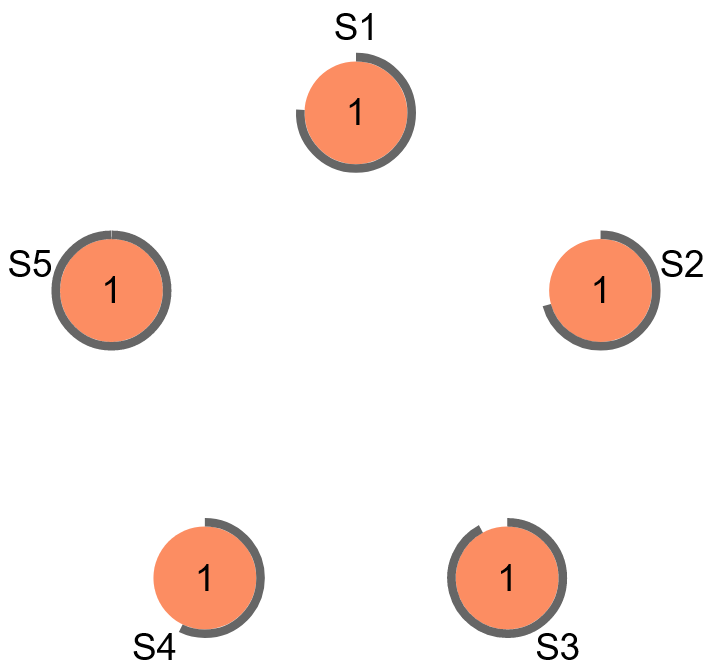
\includegraphics[width=0.45 \linewidth]{img/state_1.png}
        \label{fig:state_1}
    }
    \hfill
    \subfloat[]{
        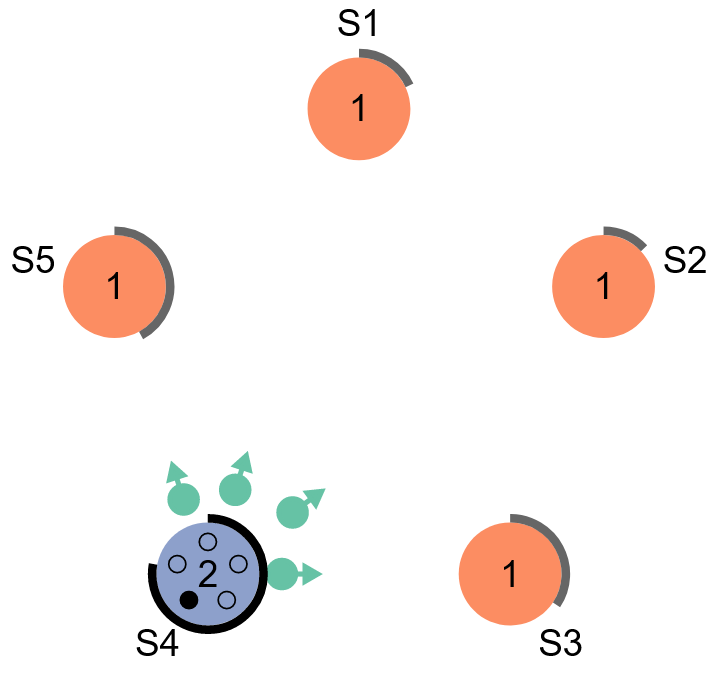
\includegraphics[width=0.45 \linewidth]{img/state_2.png}
        \label{fig:state_2}

    }
    \caption{Kai tarp mazgų nėra lyderio, mazgas, kurio rinkimų laikas yra ankščiausiai (\textit{S4}), pirmas inicijuoja naujus rinkimus ir tampa kandidatu.}
\end{figure}

Kai ateina rinkimų laikas, mazgas tampa kandidatu ir yra pradedami nauji lyderio rinkimai. \textit{S4} padidina savo terminą, balsuoja šiame rinkimų termine už save ir išsiunčia kitiems mazgams (\textit{S1}, \textit{S2}, \textit{S3}, \textit{S5}) prašymą balsuoti už jį. Prie šios užklausos yra pridedama informacija apie \textit{S4} žurnalą, kad mazgai galėtų nuspręsti, ar kandidatas \textit{S4} yra tinkamas lyderis ir ar jam reikia atiduoti savo balsą. Mazgui \textit{S4} reikia surinkti tris iš penkių balsų, taip užtikrinus daugumos pritarimą. Paveikslėlyje \ref{fig:state_2} surinkti balsai pavaizduoti kaip užtušuoti juodi apskritimai viduje mazgo.

\begin{figure}[H]
\centering
    \subfloat[]{
        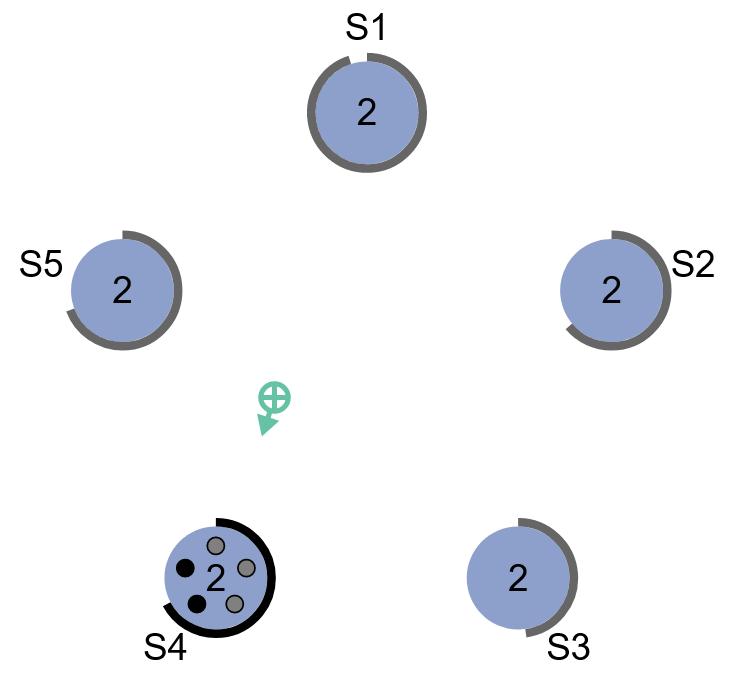
\includegraphics[width=0.45 \linewidth]{img/state_3.png}
        \label{fig:state_3}
    }
    \hfill
    \subfloat[]{
        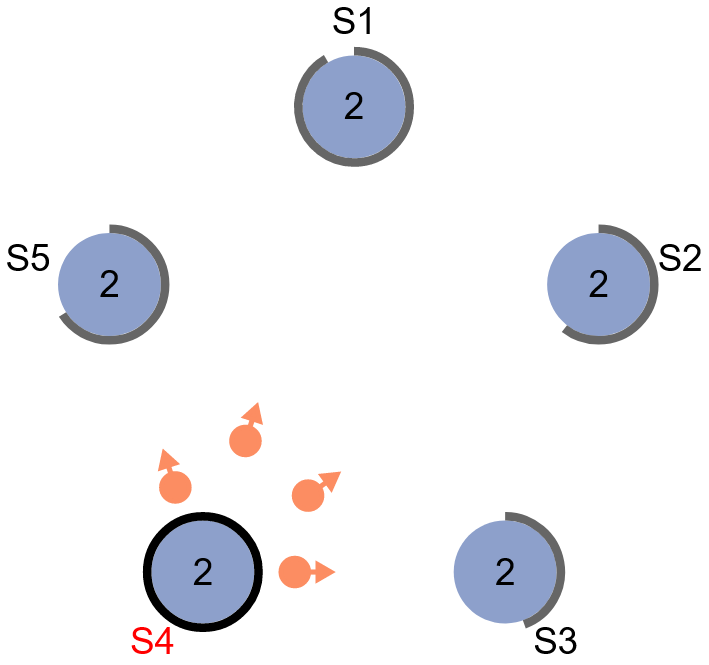
\includegraphics[width=0.45 \linewidth]{img/state_4.png}
        \label{fig:state_4}
    }
    
    \caption{Gavus daugumą balsų, mazgas--kandidatas (\textit{S4}) tampa lyderiu.}

\end{figure}

\ref{fig:state_3} \textit{S4} jau surinko du balsus -- vieną iš savęs, kitą iš kito mazgo. Gavus trečią, paskutinį reikalingą, balsą, \textit{S4} tampa lyderiu ir išsiunčia kitiems mazgams savo širdies plakimo užklausą (žr. pav. \ref{fig:state_4}). Gavus lyderio užklausą, kiti mazgai iš naujo nustato rinkimų laiką. 

\subsection{Raft įrašų perdavimas}

Išrinktas lyderis aptarnauja klientus; jei užklausas iš klientų gauna mazgas kuris nėra lyderis, jis persiunčia užklausą lyderiui. Iš kliento lyderis gauna užklausą su nusakytu veiksmu, kurį reikia atlikti paskirstytai sistemai kaip būsenų mašinai. Gautą žinutę lyderis prideda į savo žurnalą kaip naują įrašą, tada asinchroniškai išsiunčia įrašo pridėjimo užklausas sekėjams. Kai dauguma sekėjų sėkmingai prideda įrašą į savo žurnalą, įrašas yra pažymimas kaip užfiksuotas (angl. \textit{committed}), įvykdomas atitinkamas įrašo veiksmas mazgų būsenų mašinoms ir lyderis grąžina rezultatą klientui~\cite{ongaro_consensus}. 

Net jei dalis mazgų nustojo veikti ar lėtai grąžina atsakymus, lyderis pakartotinai siunčia įrašų pridėjimo užklausas tiems sekėjams, kurie dar nepatvirtino įrašo gavimo. Galiausiai visi mazgai turės visus žurnalo įrašus. Šis pakartotinio informacijos siuntimo procesas gali vykti net jau lyderiui išsiuntus atsakymą klientui. Tai užtikrina sistemos gyvybingumą kai mažesnioji dalis mazgų yra nepasiekiami~\cite{ongaro_consensus}.

\subsection{Raft mazgų tinklo trūkių neigiamų pasekmių sumažinimas}

Pagal klasikinį Raft, nutikus mazgų tinklo trūkiui, tai yra kai dalis mazgų tampa nepasiekiama kitai daliai mazgų, įvyksta papildomas lyderio išrinkimas -- atsijungusi dalis mazgų nepasiekia buvusio lyderio ir, praėjus rinkimų laikui, pradeda naują terminą (padidina kadencijos numerį). Kaip pasekmė, susijungus šioms mazgų dalims atgal į vieną tinklą, didesnė dalis mazgų gauna užklausas iš mažesnės dalies mazgų, kuriuose nurodytas terminas yra didesnis. Tada didesnės dalies mazgų lyderis atsistatydina, ir prasideda nauji rinkimai~\cite{ongaro_consensus}. Per trūkio laiką nauji įrašai galėtų būti užfiksuoti tik didesnėje dalyje mazgų, nes mažesnėje nebūtų galima gauti daugumos patvirtinimo. Jeigu per trūkio laiką buvo užfiksuota naujų įrašų, tai reikštų kad lyderiu galėtų būti išrinktas tik vienas iš tos didesnės mazgų grupės narių. Vienas iš šitų mazgų yra trūkio pabaigoje esantis lyderis. Taigi, yra vykdomi papildomi rinkimai, nors galėtų būti paliktas esamas lyderis.

Šioms klasterių apjungimo pasekmėms pašalinti Raft autoriai siūlo padaryti algoritmo praplėtimą: įvesti dar vieną mazgų būseną tarp "sekėjo" ir "kandidato" būsenų -- "pirminis balsavimas" (angl. \textit{pre-vote}). Šioje būsenoje kandidatas pradeda lyderio rinkimus tik sužinojęs, kad dauguma mazgų balsuotų už jį kaip lyderį. Mazgo terminas šioje būsenoje nėra padidinamas. Šis sprendimas išsprendžia trikdžius daliai mazgų prisijungiant atgal į didesnį mazgų klasterį, nes mažesnėje dalyje mazgų niekada nebus padidintas kadencijos numeris~\cite{ongaro_consensus}.

\section{Raft algoritmo įgyvendinimas Ra}

Šioje dalyje yra apžvelgiamas Raft algoritmo įgyvendinimas Ra. Ra yra atviro kodo Raft algoritmo biblioteka, naudojama atviro kodo žinučių brokeryje RabbitMQ\footnote{https://www.rabbitmq.com/}. Ra biblioteka yra naudojama RabbitMQ komandos paskirstytoms eilėms įgyvendinti, tačiau yra laisvai prieinama ir gali būti naudojama kaip bendra Raft biblioteka. Ra yra įgyvendinta Erlang\footnote{https://www.erlang.org/} kalba.

Nors didžioji dalis Raft algoritmo savybių yra įgyvendintos pagal Raft specifikaciją, dėl Erlang kalbos ypatybių ir konkrečių naudojimo scenarijų Ra išsiskiria nuo specifikacijos, pavyzdžiui, žurnalo perdavimo ir gedimų aptikimo algoritmais~\cite{rabbitmqra}.

Pirmoje dalyje apžvelgsime Erlang kalbos ypatybes, kurios nulėmė Ra pasirinktus įgyvendinimo sprendimus. Antroje dalyje apžvelgsime Raft praplėtimus, padarytus Ra bibliotekoje. Trečioje dalyje yra detaliau išnagrinėjamas Ra naudojamas klaidų aptikimo mechanizmas ir jis yra palyginamas su Raft pasiūlytų širdies plakimo mechanizmu naudojant \texttt{AppendEntries} užklausas.

\subsection{Paskirstytas programavimas Erlang}

Erlang yra funkcinė programavimo kalba leidžianti kurti paskirstytas, atsparias gedimams, ir didelio prieinamumo reikalaujančias sistemas. Pavadinimas ,,Erlang'' gali būti naudojamas kaip sinonimas ,,Erlang/OTP'', kur OTP (angl. \textit{Open Telecom Platform}, šiame darbe naudojame anglišką santrumpą) yra karkasas skirtas supaprastinti skirtingų sistemų bendrų bruožų įgyvendinimą; OTP yra prieinamas kartu su Erlang kalba ir yra standartinės bibliotekos, kaip kalbos C++ bibliotekos \texttt{std}, atitikmuo~\cite{erlang_introduction}. Šiame darbe autoriai naudoja pavadinimą ,,Erlang'' tik Erlang programavimo kalbai vadinti.

Paskirstytas programavimas Erlang yra pagrįstas aktorių modeliu~\cite{farrugia_towards_nodate, agha_actors_1985}. Pagrindinis Erlang vykdymo vienetas yra mazgas (angl. \textit{node}) -- tai yra Erlang virtualios mašinos vienetas (paskirstytos sistemos vienetus taip pat vadinsime mazgais). Erlang mazgas gali turėti tūkstančius jame vykdomų procesų (angl. \textit{process}), o procesai komunikuoja vienas su kitu žinučių pagalba (angl. \textit{message}). Jeigu vienas iš procesų nustos veikti, tai neįtakoja kitų procesų ir jie tęsia savo darbą. Nenumatytoms klaidoms suvaldyti procesai gali būti prižiūrimi prižiūrėtojo (angl. \textit{supervisor}), kuris gautų pranešimą nenumatytai klaidai įvykus ir prižiūrimam procesui nustojus veikti~\cite{erlang_distributed}.

Erlang mazgai gali būti paskirstyti per daugiau negu vieną mašiną ir bendrauja vienas su kitu tranzityvinių ryšiu pagalba. Kai vienas iš mazg sudaro ryšį su kitu mazgu (pavyzdžiui, panaudojus \texttt{net\_kernel:connect/1}), mazgai apsikeičia žinomais mazgais ir taip sudaro vieną mazgų tinklą. Erlang mazgų sistema yra labai lanksti ir leidžia vienam iš mazgų deleguoti kitam mazgui laisvai pasirinktą funkciją vykdymui (angl. \textit{arbitrary code execution}). \texttt{net\_kernel} modulio pagalba vienas iš mazgų gali prenumeruoti mazgų statusų pakeitimų žinučių gavimą. Tokiu atveju, pasikeitus žinomo mazgo statusui, prenumeravęs mazgas gaus pranešimą su nauju mazgo statusu~\cite{erlang_distributed, hebert_learn_2013}. Ra bibliotekos atveju, didžiausią sistemos prieinamumą suteiks nelyginio skaičiaus mašinų su vienu Erlang mazgu vykdančių Ra kodą kiekvienoje mašinoje paskirstytos sistemos architektūra.

Erlang mazgai palaiko ryšį tarp vienas kito "širdies plakimo" (angl. \emph{heartbeat}) mechanizmo pagalba. \texttt{ticktime} yra širdies plakimo užklausos siuntimo intervalas padaugintas iš keturių ir žymi laiką, po kurio mazgas bus laikomas nepasiekiamu. Kai vienas iš mazgų negauna iš kito mazgo jo gyvavimo patvirtinančio pranešimo per \texttt{ticktime} sekundžių, tas stebimas mazgas laikomas nepasiekiamu. Širdies plakimo užklausos neišsiuntimo priežastimi gali būti kaip ir techninės įrangos gedimai ir ryšio sutrikimai, taip ir mazgo siuntimo kanalo didelis užimtumas -- Erlang naudoja tą patį TCP (angl. \emph{Transmission Control Protocol}) kanalą naudotojo aprašytoms ir širdies plakimo žinutėms siųsti, todėl didelių žinučių siuntimas gali priversti širdies plakimo žinutes ilgai laukti savo eilės~\cite{hebert_learn_2013}.

\subsection{Ra įgyvendinti Raft algoritmo praplėtimai}

Dėl Erlang kalbos ypatybių, konkretaus naudojimo scenarijaus ir siekio optimizuoti Raft algoritmo veikimo laiką ir naudojamų duomenų kiekį, Ra išsiskiria nuo specifikacijos kelių savybių įgyvendinimu~\cite{rabbitmqra}. Šiame skyriuje yra pateikiama Ra žurnalo perdavimo algoritmo ir Ra mazgų negyvybingumo aptikimo mechanizmų apžvalgos. 

\subsubsection{Ra žurnalo perdavimo algoritmas}

Ra nenaudoja žurnalo įrašų perdavimo užklausų mazgų gyvybingumui užtikrinti kai visų mazgų žurnalai yra sinchronizuoti. Kai vienas iš mazgų yra pasenęs, tai yra, to mazgo paskutinis sinchronizuotas įrašas yra ankstesnis negu paskutinis įrašas, siųstas lyderio tam mazgui, \texttt{AppendEntries} užklausa yra daroma, bet rečiau, negu pasiūlyta Raft specifikacijoje. Jei skirtumas tarp paskutinio sinchronizuoto įrašo ir paskutinio siųsto įrašo yra labai didelis, mazgo apkrovai sumažinti užklausos nėra siunčiamos~\cite{rabbitmqra}. Žurnalų įrašų perdavimas yra vykdomas asinchroniškai, o atsakymai yra grupuojami~\cite{rabbitmqra}.

Šiuo praplėtimo atveju Ra autoriai išnaudojo Erlang kalbos galimybes, nes Erlang leidžia palaikyti ryšį tarp mazgų išreikštinai nesiunčiant papildomų užklausų. Nesiunčiant papildomų užklausų taip pat yra atlaisvinamas ryšio kanalas, leidžiant pačiam Erlang efektyviai palaikyti ryšius ir daryti širdies plakimo užklausas. Taigi, Ra funkcionalumas atitinka Raft specifikaciją. Dėl šitos priežasties galima teigti, kad Ra autoriai laikėsi Raft specifikacijos ir nepažeidė Raft nustatytų algoritmo savybių praplečiant žurnalo perdavimo algoritmą.      

\subsubsection{Ra gedimų aptikimo algoritmas}

Ra nenaudoja Raft aprašyto gedimo aptikimo algoritmo. Ra naudoja gimtąjį Erlang mazgų stebėjimo infrastruktūrą stebėti ar mazgai nenustojo veikti ir kartu pasitelkia Aten\footnote{https://github.com/rabbitmq/aten} biblioteka mazgų susisiekimo klaidoms aptikti~\cite{rabbitmqra}. Aten yra adaptyvus kaupiamasis gedimų aptikimo algoritmas, kuris atsižvelgia į širdies plakimų istoriją ir pagal tai nusprendžia, ar yra didelė tikimybė nesulaukti sekančio gyvumo patvirtinimo. Tai yra naudinga siekiant sumažinti klaidingai teigiamų gedimo rezultatų skaičių didelio tinklo apkrovos metu~\cite{satzger2007_new_accrual_failure}.  

Gimtieji Erlang monitoriai leidžia greitai aptikti mazgų neveikimą proceso lūžio atveju (angl. \textit{crash}). Stebėtojui yra išsiunčiama \texttt{'DOWN'} žinutė~\cite{ericsson_erlang_processes_2016}. Erlang monitoriai užtikrina greitą lyderio mazgo neveikimo aptikimą jo sekėjais ir taip iš dalies pakeičia Raft širdies plakimo mechanizmą~\cite{rabbitmqra}. Aten biblioteka leidžia aptikti tinklo paskirstymo problemas, kaip mazgų nepasiekiamumą per tinklą. Kai Aten įtaria kad vienas iš mazgų yra nepasiekiamas, yra išsiunčiama \texttt{nodedown} žinutė mazgo stebėtojui. Atitinkamai, jei mazgas ,,atsigauna'' ir atrodo vėl veikiantis, yra išsiunčiama \texttt{nodeup} žinutė~\cite{rabbitmq_aten_2020}. Kartu Erlang monitoriai ir Aten biblioteka, anot Ra autorių, užtikrina mazgų gyvumą ir pakeičia Raft aprašytą širdies plakimo mechanizmą~\cite{rabbitmqra}. 

Ra bibliotekoje visi mazgai kurie naudoja Raft algoritmą yra įgyvendinti kaip būsenų mašinos Erlang modulio \texttt{gen\_statem} \footnote{http://erlang.org/doc/man/gen\_statem.html} pagalba. 
Pirmiausia būsenų mašina  prenumeruoja gauti pranešimus apie mazgų statusų pokyčius su \texttt{net\_kernel:monitor\_nodes/1}\footnote{http://erlang.org/doc/man/net\_kernel.html\#monitor\_nodes-1}. Kai vienas iš mazgų tampa neprieinamas, mazgas gauna \texttt{'DOWN'} pranešimą ir įvykdo atitinkamą Raft algoritmo logiką. Neprieinamumo tikrinimo laiką \texttt{ticktime} naudotojas nustato pagal savo poreikį konfigūracinio parametro pagalba~\cite{rabbitmqra}.

Taigi, Ra naudoja Erlang monitorius kiekvieno iš mazgų būsenoms stebėti. Tai leidžia palengvinti įgyvendinimo kaštus, nes didžioji dalis širdies plakimo mechanizmo algoritmo yra paimama iš Erlang OTP bibliotekos. Mazgui netikėtai nustojus veikti, klaida bus aptikta iškarto, o mazgui lėtai atsakant ar ryšiui nutrūkus, širdies plakimo mechanizmas atitinka Raft specifikaciją ir išsaugo Raft savybes.

\section{Ra gedimų aptikimo algoritmo formali specifikacija}

Šioje dalyje yra pateikiama formali Ra gedimų aptikimo algoritmo specifikacija, parašyta TLA$^+$ kalba.

apie TLA Plius

- Timed out but then came back?


\sectionnonum{Rezultatai ir išvados}

Šiame darbe buvo išnagrinėtas Raft algoritmas ir jo įgyvendinimas -- Ra biblioteka. Detaliau buvo palyginti Raft darbe aprašyti mazgų negyvybingumo aptikimo algoritmai su Ra naudojamais Erlang mazgų stebėjimo infrastruktūra. Nustatyta, kad Raft pasiūlytas mechanizmas, ir Ra naudojamas Erlang gimtasis funkcionalumas, yra to paties širdies plakimo algoritmo įgyvendinimai ir esminių skirtumų tarp jų nėra. Todėl teigiama, kad Ra įgyvendinimas yra korektiškas ir išlaiko Raft savybes.

Erlang Raft algoritmo įgyvendinimas Ra yra gerokai palengvinamas tuo, kad gimtosios Erlang funkcijos ir bibliotekos yra skirtos būtent tokių paskirstytų sistemų būsenų stebėjimui, todėl įgyvendinimo kaštai yra dar labiau sumažinami. Visa tai gerai komponuoja su Raft autorių motyvacija~\cite{ongaro_consensus} -- padaryti paskirstytų sistemų konsensuso algoritmo įgyvendinimą kuo paprastesnį, sumažinti galimų klaidų skaičių, leisti kuo lengviau papildyti esamą funkcionalumą naujais praplėtimais. Šio darbo autorių nuomone, Ra biblioteka yra ne tik puikus techninio Raft algoritmo įgyvendinimo, bet ir Raft paprastumo ir aiškumo dvasią išlaikančios bibliotekos pavyzdys. 

%Rezultatų ir išvadų dalyje turi būti aiškiai išdėstomi pagrindiniai darbo
%rezultatai (kažkas išanalizuota, kažkas sukurta, kažkas įdiegta) ir pateikiamos
%išvados (daromi nagrinėtų problemų sprendimo metodų palyginimai, teikiamos
%rekomendacijos, akcentuojamos naujovės).

\printbibliography[heading=bibintoc]  % Šaltinių sąraše nurodoma panaudota
% literatūra, kitokie šaltiniai. Abėcėlės tvarka išdėstomi darbe panaudotų
% (cituotų, perfrazuotų ar bent paminėtų) mokslo leidinių, kitokių publikacijų
% bibliografiniai aprašai.  Šaltinių sąrašas spausdinamas iš naujo puslapio.
% Aprašai pateikiami netransliteruoti. Šaltinių sąraše negali būti tokių
% šaltinių, kurie nebuvo paminėti tekste.

% \sectionnonum{Sąvokų apibrėžimai}
% \sectionnonum{Santrumpos}
%Sąvokų apibrėžimai ir santrumpų sąrašas sudaromas tada, kai darbo tekste
%vartojami specialūs paaiškinimo reikalaujantys terminai ir rečiau sutinkamos
%santrumpos.

\appendix  % Priedai

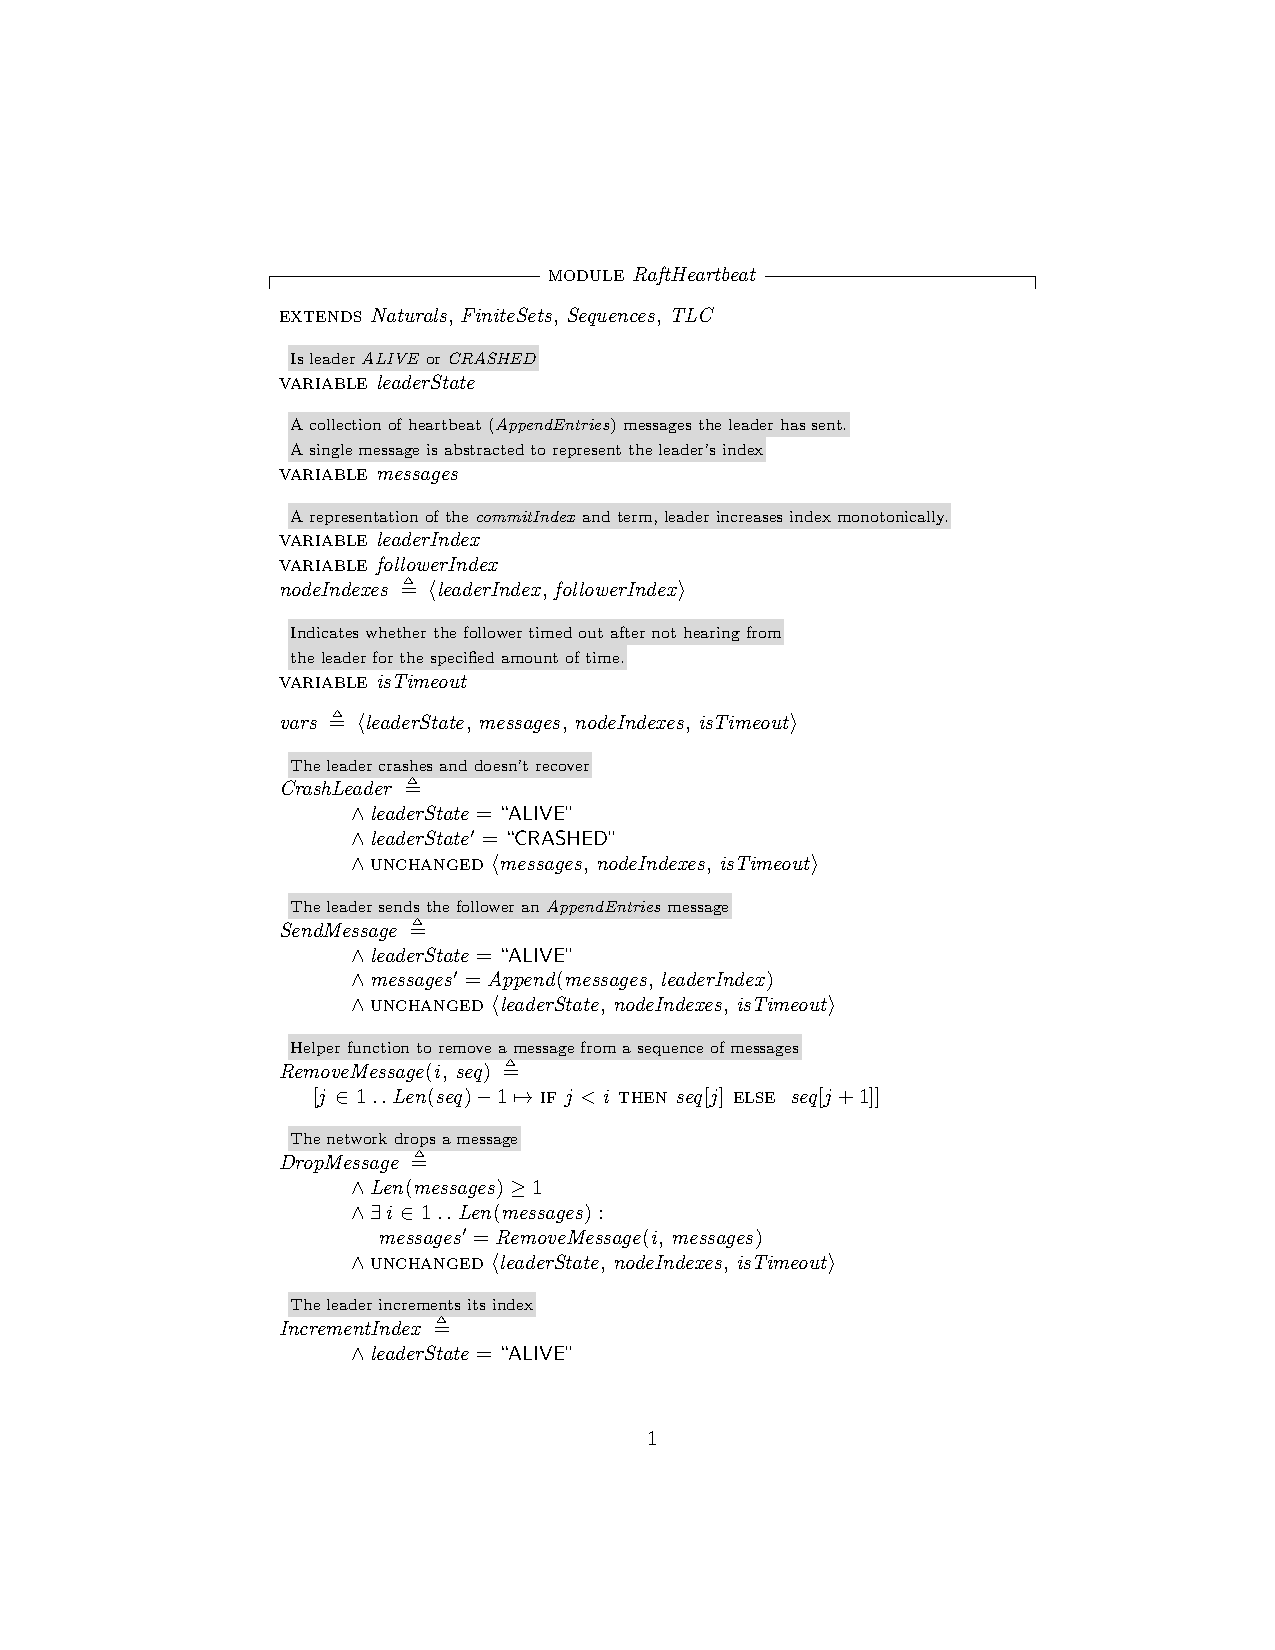
\includepdf[pages=1, pagecommand=\section{Raft algoritmo gedimo aptikimo specifikacija TLA$^+$ kalba}\label{sec:appendix_raft_tla_spec}]{spec/RaftHeartbeat.pdf}
\includepdf[pages=2-]{spec/RaftHeartbeat.pdf}

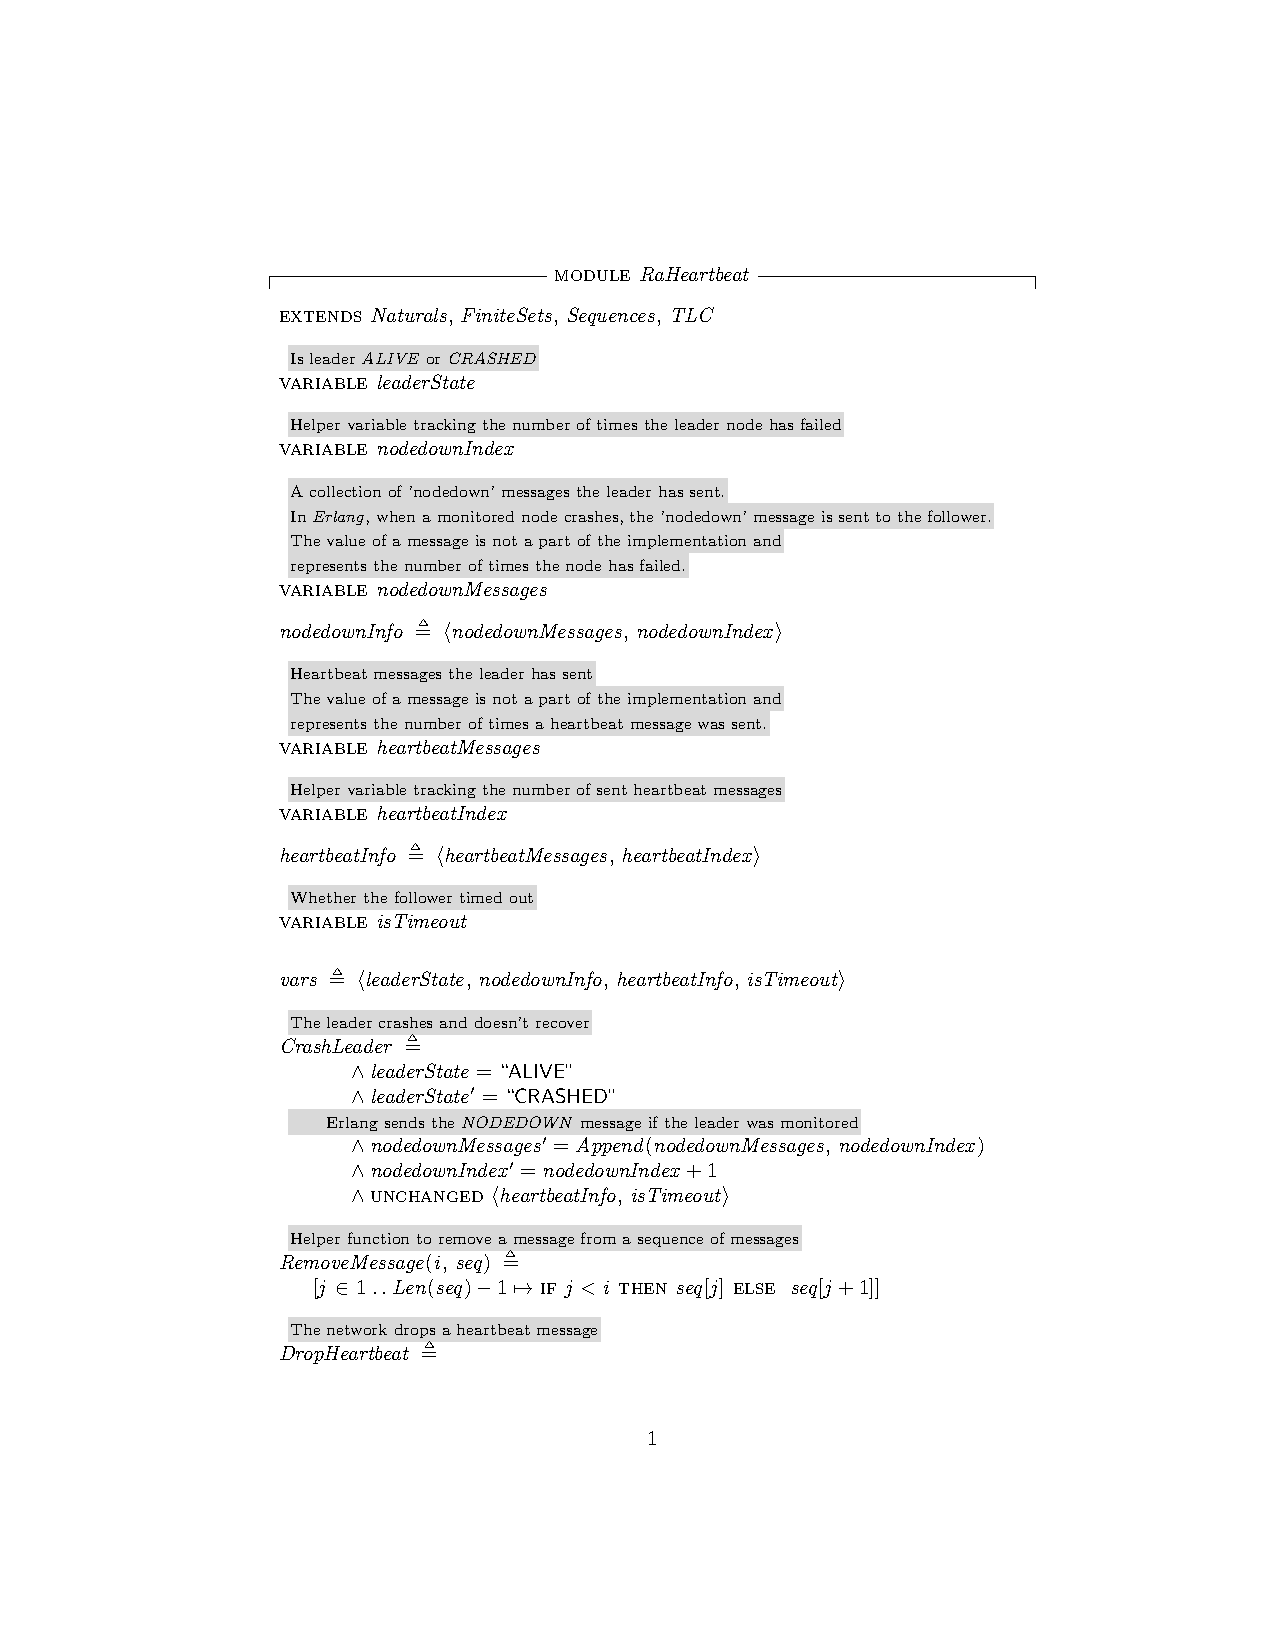
\includepdf[pages=1, pagecommand=\section{Ra bibliotekos gedimo aptikimo specifikacija TLA$^+$ kalba}\label{sec:appendix_ra_tla_spec}]{spec/RaHeartbeat.pdf}
\includepdf[pages=2-]{spec/RaHeartbeat.pdf}

% Prieduose gali būti pateikiama pagalbinė, ypač darbo autoriaus savarankiškai
% parengta, medžiaga. Savarankiški priedai gali būti pateikiami ir
% kompaktiniame diske. Priedai taip pat numeruojami ir vadinami. Darbo tekstas
% su priedais susiejamas nuorodomis.

\end{document}
